\chapter{半導体の物理}
\label{chap1}

序章で見たとおり，電力変換の主役はエネルギーの流れ道を高速に切り替える半導体スイッチである。
本章では，そのスイッチの材料である半導体を物理から解き明かす。
遠回りに見えるが，ここで登場する量が後の章の設計判断を支える。
たとえばバンドギャップの大きさが素子の耐圧と高温動作を決め（3章），
キャリアの動きやすさがオン抵抗と導通損失を決める（3章，5章）。

本章ではまず半導体とはどんな物質かを整理し（\ref{sec1.1}節），
電子が原子の中でとびとびのエネルギーしか取れないことを確認する（\ref{sec1.2}節）。
そのうえで固体中の電子をバンドで説明し（\ref{sec1.3}節），
不純物でキャリアの数を自在に操れること（\ref{sec1.4}節），
キャリアが動く2つのしくみ（\ref{sec1.5}節）を学ぶ。
最後に，すべての半導体素子の出発点であるpn接合（\ref{sec1.6}節）と
金属-半導体接合（\ref{sec1.7}節）の物理を，電磁気の言葉で読み解く。

\begin{screen}
\noindent\textbf{この章の量が後で効く場所}\\[3pt]
\begin{箇条書}
\item バンドギャップ$E_g$ → 漏れ電流・高温動作・絶縁破壊電界（3章，SiC・GaN）
\item 移動度$\mu$とドーピング濃度 → オン抵抗（3章）・導通損失（5章）
\item 空乏層 → 耐圧（3章）・接合容量とスイッチング（2章）
\end{箇条書}
\end{screen}

%%======================================================================
\section{半導体とは何か}
\label{sec1.1}

\subsection{スイッチとしての半導体}

パワーエレクトロニクスで半導体素子に求められる仕事は，理想的には次の4つである。

\begin{箇条書}
\item \textbf{オン状態}：抵抗ゼロで大電流を流す
\item \textbf{オフ状態}：抵抗無限大で電流を完全に断つ
\item \textbf{高速動作}：オンとオフを高速に切り替える
\item \textbf{低損失}：切り替えのときのエネルギー損失が小さい
\end{箇条書}

実際の素子はこの理想には届かないが，機械式のスイッチに比べて圧倒的に速く，
接点の摩耗もない。
「電流を流したり止めたりできる」という性質はどこから来るのか。
その答えが本章の主題である。

\subsection{導体・半導体・絶縁体}

物質は電気の流れやすさで大きく3つに分けられる。

\begin{箇条書}
\item \textbf{導体}\index{どうたい@導体}：電流が非常に流れやすい。銅，アルミニウム，金など
\item \textbf{絶縁体}\index{ぜつえんたい@絶縁体}：電流がほとんど流れない。ガラス，ゴム，酸化シリコンなど
\item \textbf{半導体}\index{はんどうたい@半導体}：両者の中間。シリコン，ゲルマニウム，炭化シリコンなど
\end{箇条書}

\textbf{半導体}の特長は，単に「中間の抵抗をもつ」ことではない。
温度・不純物・電圧といった外部条件によって，
\textbf{電流を流すか流さないかを制御できる}ことである。
この性質があるからこそ，半導体はスイッチになれる。

\subsection{電流はキャリアの移動である}

電流$I$は，単位時間に断面を通過する電荷$Q$の量である。
\begin{equation}
I = \frac{dQ}{dt}
\label{eq1.1}
\end{equation}
電荷を運ぶ粒子を\index{きゃりあ@キャリア}\textbf{キャリア}という。
半導体のキャリアは電子（電荷$-e$）と，後で導入する正孔（電荷$+e$）である。
ここで$e = 1.602\times10^{-19}$\,Cは\index{でんきそりょう@電気素量}電気素量である。
つまり導体・半導体・絶縁体の違いは，
\textbf{動けるキャリアがどれだけあるか}の違いにほかならない。
動けるキャリアの数を決めるしくみを知るには，
まず電子が物質の中でどんなエネルギーを取れるのかを知る必要がある。

\begin{問}
\item スイッチング素子に$10$\,Aの電流が流れている。
1秒間に素子の断面を通過する電子の数を求めよ。
\end{問}

%%======================================================================
\section{原子構造と電子配置}
\label{sec1.2}

\subsection{電子はとびとびのエネルギーしか取れない}

すべての物質は原子からできている。
原子は正電荷をもつ\textbf{原子核}と，その周りの\textbf{電子}からなる。
電子は原子核の周りに勝手な軌道を描くのではなく，
決まった\index{きどう@軌道（電子）}\textbf{軌道}にしか存在できない。
軌道は内側からK殻，L殻，M殻，$\cdots$という\index{でんしかく@電子殻}\textbf{電子殻}にまとめられ，
各殻はさらに細かい軌道（s軌道，p軌道など）に分かれる。
1つの軌道に入れる電子は最大2個である（パウリの排他原理）。

重要なのは，\textbf{各軌道が固有のエネルギーをもつ}ことである。
電子が取れるエネルギーはとびとびの値（エネルギー準位）に限られ，
電子は低い準位から順に詰まっていく。
低いエネルギーの状態ほど安定だからである。

\subsection{シリコンの電子配置と価電子}

パワーエレクトロニクスで最も広く使われる半導体はシリコン（Si，原子番号14）である。
14個の電子は低い準位から順に詰まり，電子配置は次のようになる。
\begin{equation*}
\mathrm{Si:}\ 1s^2\,2s^2\,2p^6\,3s^2\,3p^2
\end{equation*}
最も外側のM殻には$3s^2\,3p^2$の4個の電子があり，
これを\index{かでんし@価電子}\textbf{価電子}という。
価電子が4個の元素を4価の元素という。
シリコン結晶では，各原子が隣の4個の原子と価電子を1個ずつ出し合って結び付き
（共有結合），すべての価電子が結合に使われた安定な構造を作る。
化学結合も電気伝導も，この一番外側の価電子が担う。

\begin{問}
\item リン（P，原子番号15）とホウ素（B，原子番号5）の電子配置を書き，
それぞれの価電子の数を答えよ。
\end{問}

%%======================================================================
\section{バンド理論}
\label{sec1.3}

\subsection{準位がバンドになる}

孤立した1個の原子では，電子のエネルギー準位はとびとびである。
ところが原子が近づくと電子の軌道が重なり合い，
同じだった準位がわずかに異なる多数の準位に分裂する。
固体では$1\,\mathrm{cm}^3$あたり約$5\times10^{22}$個（シリコンの場合）もの原子が集まるから，
準位は事実上すき間なく並び，幅をもった帯とみなせる。
これを\index{えねるぎーばんど@エネルギーバンド}\textbf{エネルギーバンド}という。
固体中の電子はこのバンドの中のエネルギーしか取れない。

\begin{定義}[価電子帯・伝導帯・バンドギャップ]
\label{def1.1}
\begin{箇条書}
\item \index{かでんしたい@価電子帯}\textbf{価電子帯}：価電子が占めるバンド。低温では電子でほぼ満ちている
\item \index{でんどうたい@伝導帯}\textbf{伝導帯}：その上にある，電子が自由に動き回れるバンド
\item \index{ばんどぎゃっぷ@バンドギャップ}\textbf{バンドギャップ}$E_g$：両バンドの間の，電子が存在できないエネルギーの幅
\end{箇条書}
\end{定義}

満ちた価電子帯の電子は動けない。
すべての席が埋まった満員電車の中で人が移動できないのと同じで，
移動先の空きがないからである。
電流を運べるのは，伝導帯に上がった電子と，
価電子帯にできた空席（正孔，後述）だけである。

\subsection{バンドで見る導体・半導体・絶縁体}

物質の電気的性質は，バンドの構造で決まる（\FIGref{fig1.1}）。

\begin{figure}[ht]
\begin{center}
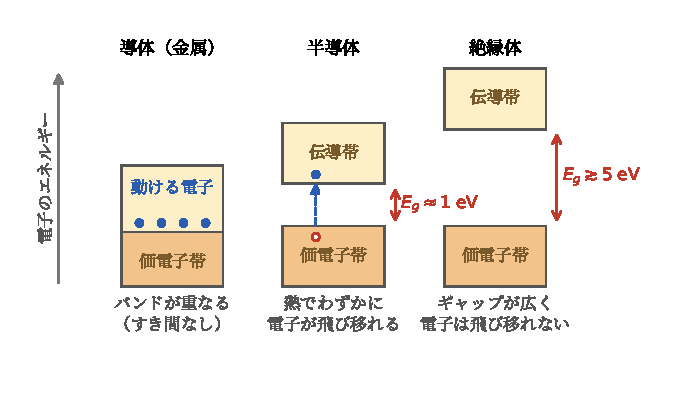
\includegraphics[clip]{figures/fig1.1.eps}
\end{center}
\caption{導体・半導体・絶縁体のバンド構造。バンドギャップの大きさが電気の流れやすさを決める}
\label{fig1.1}
\end{figure}

\begin{箇条書}
\item \textbf{導体}：価電子帯と伝導帯が重なる，または伝導帯に最初から電子がある。
動ける電子が常に多数あり，電流がよく流れる
\item \textbf{絶縁体}：$E_g$が大きい（おおむね5\,eV以上）。
室温の熱エネルギーでは電子が伝導帯に上がれず，電流はほとんど流れない
\item \textbf{半導体}：$E_g$が小さい（おおむね0.5〜3.5\,eV）。
室温でもわずかに電子が伝導帯へ上がり，外部条件でその数を制御できる
\end{箇条書}

代表的な半導体のバンドギャップを挙げる。

\begin{箇条書}
\item シリコン（Si）：$E_g \approx 1.1$\,eV
\item ゲルマニウム（Ge）：$E_g \approx 0.67$\,eV
\item 炭化シリコン（SiC）：$E_g \approx 3.3$\,eV
\item 窒化ガリウム（GaN）：$E_g \approx 3.4$\,eV
\end{箇条書}

SiCとGaNは，シリコンの約3倍のバンドギャップをもつため
\index{わいどぎゃっぷはんどうたい@ワイドギャップ半導体}\textbf{ワイドギャップ半導体}と呼ばれる。
バンドギャップが大きいほど熱でキャリアが生まれにくく（漏れ電流が小さく，高温に強い），
後述の絶縁破壊電界も大きい（薄い層で高電圧に耐えられる）。
この2つの利点が高耐圧・低損失のパワーデバイスに直結することを3章で見る。

\begin{注意}
eV（エレクトロンボルト）\index{えれくとろんぼると@エレクトロンボルト}は
電子1個が$1$\,Vの電位差で得るエネルギーで，
$1\,\mathrm{eV} = 1.602\times10^{-19}$\,Jである。
バンドギャップのような電子1個のエネルギーはJでは小さすぎるため，本書ではeVを使う。
\end{注意}

\subsection{フェルミ準位とフェルミ・ディラック分布}

固体には膨大な数の電子があるから，1個ずつ追いかけるのではなく，
「エネルギー$E$の状態が電子で占められている確率$f(E)$」で統計的に扱う。
この確率は\index{ふぇるみでぃらっくぶんぷ@フェルミ・ディラック分布}\textbf{フェルミ・ディラック分布}で与えられる。
\begin{equation}
f(E) = \frac{1}{1 + \exp\left(\dfrac{E - E_F}{kT}\right)}
\label{eq1.2}
\end{equation}
ここで$k = 1.381\times10^{-23}$\,J/K（$= 8.62\times10^{-5}$\,eV/K）は
\index{ぼるつまんていすう@ボルツマン定数}ボルツマン定数，$T$は絶対温度である。

\begin{定義}[フェルミ準位]
\label{def1.2}
\index{ふぇるみじゅんい@フェルミ準位}\textbf{フェルミ準位}$E_F$は，
電子で占められる確率がちょうど$1/2$になるエネルギーである。
$E_F$より十分低い準位はほぼ満ち（$f \approx 1$），
十分高い準位はほぼ空である（$f \approx 0$）。
\end{定義}

室温（$T = 300$\,K）では$kT \approx 0.026$\,eVである。
不純物を含まない半導体では$E_F$はバンドギャップのほぼ中央にあり，
伝導帯の下端はそこから$E_g/2$（シリコンで約$0.55$\,eV）も上にある。
$kT$の20倍以上だから占有確率はきわめて小さいが，ゼロではない。
室温の半導体がわずかに電流を流すのは，
この分布のすそが伝導帯に届いているからである。

\subsection{正孔}

熱で電子が価電子帯から伝導帯へ上がると，価電子帯に空席が1つ残る。
この空席を\index{せいこう@正孔}\textbf{正孔}という。
空席があれば隣の電子がそこへ移れ，移った跡にまた空席ができる。
電子が次々に動く様子は，\textbf{空席が逆向きに動く}様子として追いかける方が簡単である。
正孔は電荷$+e$をもつ1つのキャリアとして扱え，電場と同じ向きに動く。

\begin{注意}
正孔は実在の粒子ではなく，「電子の抜けた穴」に名前を付けたものである。
しかし電荷$+e$の粒子とみなして電流を計算してよいことが知られており，
以降は電子と正孔を対等な2種類のキャリアとして扱う。
\end{注意}

\begin{問}
\item 室温（$kT = 0.026$\,eV）で，フェルミ準位より$0.55$\,eV高い準位が
電子で占められる確率を式\ref{eq1.2}から概算せよ。
$\exp\left(\frac{E-E_F}{kT}\right) \gg 1$を利用してよい。
\end{問}

%%======================================================================
\section{真性半導体と不純物半導体}
\label{sec1.4}

\subsection{真性半導体}

不純物を含まない純粋な半導体を
\index{しんせいはんどうたい@真性半導体}\textbf{真性半導体}という。
真性半導体では電子と正孔は必ず対で生まれるから，両者の濃度は等しい。
この濃度を\index{しんせいきゃりあのうど@真性キャリア濃度}\textbf{真性キャリア濃度}$n_i$といい，
室温のシリコンでは$n_i \approx 1.5\times10^{10}\,\mathrm{cm^{-3}}$である。
原子密度$5\times10^{22}\,\mathrm{cm^{-3}}$と比べると，
1兆個に1個よりも少ない割合しかキャリアがない。
真性半導体は，そのままではほとんど電流を流せないのである。

\subsection{ドーピング}

半導体に不純物をごく微量，意図的に混ぜることを
\index{どーぴんぐ@ドーピング}\textbf{ドーピング}という。
ドーピングする不純物は2種類ある。

\begin{箇条書}
\item \index{どなー@ドナー}\textbf{ドナー}：電子を供給する5価の元素（リンP，ヒ素Asなど）
\item \index{あくせぷた@アクセプタ}\textbf{アクセプタ}：正孔を供給する3価の元素（ホウ素B，ガリウムGaなど）
\end{箇条書}

5価の元素をシリコン結晶に入れると，価電子5個のうち4個は周囲との共有結合に使われ，
1個が余る。
余った電子はごく弱くしか束縛されず（束縛エネルギーは$0.05$\,eV程度），
室温の熱で簡単に伝導帯へ上がる。
バンド図では，ドナーは伝導帯のすぐ下に準位$E_d$を作り，
そこから電子を伝導帯へ供給する（\FIGref{fig1.2}(b)）。
こうして電子を多数もつ半導体を
\index{えぬがたはんどうたい@n形半導体}\textbf{n形半導体}という。

逆に3価の元素を入れると，共有結合を4本作るには電子が1個足りない。
価電子帯の電子がこの不足分（アクセプタ準位$E_a$）に上がると，価電子帯に正孔が残る
（\ref{fig1.2}(c)）。
正孔を多数もつ半導体を
\index{ぴーがたはんどうたい@p形半導体}\textbf{p形半導体}という。

\begin{figure}[ht]
\begin{center}
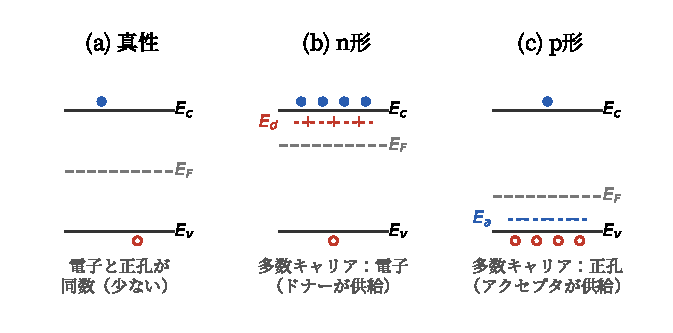
\includegraphics[clip]{figures/fig1.2.eps}
\end{center}
\caption{真性・n形・p形半導体のバンド図。ドーピングで多数キャリアの種類と数，
フェルミ準位の位置が変わる}
\label{fig1.2}
\end{figure}

数が多い方のキャリアを\index{たすうきゃりあ@多数キャリア}\textbf{多数キャリア}，
少ない方を\index{しょうすうきゃりあ@少数キャリア}\textbf{少数キャリア}という。
n形では電子が多数キャリアで，電子濃度$n$はほぼドナー濃度$N_d$に等しい。
p形では正孔が多数キャリアで，正孔濃度$p$はほぼアクセプタ濃度$N_a$に等しい。
フェルミ準位は，n形では伝導帯の近くへ，p形では価電子帯の近くへ移る
（\ref{fig1.2}）。
「電子で満ちている境目」が多数キャリアの側へ寄る，と読めばよい。

熱平衡では，電子と正孔の濃度の積はドーピングによらず一定である。
\begin{equation}
np = n_i^2
\label{eq1.3}
\end{equation}
これを\index{しつりょうさようのほうそく@質量作用の法則}\textbf{質量作用の法則}という。
多数キャリアを増やすと，少数キャリアはその分だけ減る。

\begin{例題}[ドーピングとキャリア濃度]
\label{rei1.1}
シリコンにドナーをドーピングして，
濃度$N_d = 10^{16}\,\mathrm{cm^{-3}}$のn形半導体を作った。
(a)不純物原子の割合，(b)電子濃度$n$と正孔濃度$p$を求めよ。
室温とし，シリコンの原子密度を$5\times10^{22}\,\mathrm{cm^{-3}}$，
$n_i = 1.5\times10^{10}\,\mathrm{cm^{-3}}$とする。
\begin{解答}
(a) $\dfrac{10^{16}}{5\times10^{22}} = 2\times10^{-7}$，
すなわち1000万個に2個の割合である。
(b) 多数キャリアの電子は$n \approx N_d = 10^{16}\,\mathrm{cm^{-3}}$。
少数キャリアの正孔は式\ref{eq1.3}より
\begin{equation*}
p = \frac{n_i^2}{n} = \frac{(1.5\times10^{10})^2}{10^{16}}
\approx 2.3\times10^{4}\,\mathrm{cm^{-3}}
\end{equation*}
ドーピング前の$n_i$と比べて，電子は約$10^6$倍に増え，正孔は約$10^6$分の1に減る。
1000万分の2の不純物が，キャリアの数を100万倍も変える。
これが「不純物で電気伝導を制御できる」という半導体の特長の正体である。
\end{解答}
\end{例題}

パワーデバイスでは，ドーピング濃度は$10^{13}$〜$10^{20}\,\mathrm{cm^{-3}}$の広い範囲で
場所ごとに作り分けられる。
濃度の低い層は高電圧に耐える役割（耐圧），
濃度の高い層は電流をよく流す役割（低抵抗）を受け持つ。
この作り分けがデバイス設計そのものであることを3章で見る。

\begin{問}
\item p形シリコンにアクセプタを$N_a = 10^{17}\,\mathrm{cm^{-3}}$だけドーピングした。
多数キャリアと少数キャリアはそれぞれ何か。その濃度を求めよ。
$n_i = 1.5\times10^{10}\,\mathrm{cm^{-3}}$とする。
\end{問}

%%======================================================================
\section{キャリアの輸送 ― ドリフトと拡散}
\label{sec1.5}

キャリアがあるだけでは電流にならない。キャリアが\textbf{動いて}はじめて電流になる。
キャリアが動くしくみは，ドリフトと拡散の2つしかない（\FIGref{fig1.3}）。

\begin{figure}[ht]
\begin{center}
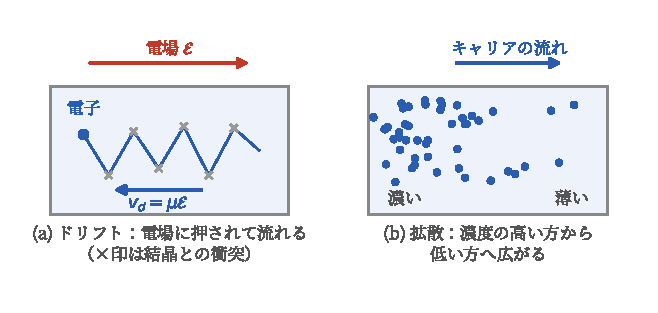
\includegraphics[clip]{figures/fig1.3.eps}
\end{center}
\caption{キャリアが動く2つのしくみ。(a)ドリフトは電場に押されて流れ，
(b)拡散は濃度の高い方から低い方へ広がる}
\label{fig1.3}
\end{figure}

\begin{注意}
バンド図ではエネルギーを$E$と書くため，
本章では電場の大きさを$\mathcal{E}$と書いて区別する。
\end{注意}

\subsection{ドリフト}

半導体に電場$\mathcal{E}$をかけると，キャリアは電場から力を受けて加速される。
ただし結晶中の原子や不純物に衝突しては向きを変えるため，
どこまでも速くなるわけではなく，平均すると一定の速度で流れる
（\ref{fig1.3}(a)）。
この流れを\index{どりふと@ドリフト}\textbf{ドリフト}，平均速度をドリフト速度$v_d$という。

\begin{定義}[移動度と導電率]
\label{def1.3}
ドリフト速度は電場に比例し，比例係数$\mu$を
\index{いどうど@移動度}\textbf{移動度}という（単位はm$^2$/(V$\cdot$s)）。
\begin{equation}
v_d = \mu \mathcal{E}
\label{eq1.4}
\end{equation}
電子濃度$n$，正孔濃度$p$の半導体を流れるドリフト電流の密度は
\begin{equation}
J = e (n \mu_n + p \mu_p) \mathcal{E} = \sigma \mathcal{E}
\label{eq1.5}
\end{equation}
と書ける。$\mu_n$，$\mu_p$は電子と正孔の移動度，
$\sigma = e(n\mu_n + p\mu_p)$を\index{どうでんりつ@導電率}\textbf{導電率}という（単位はS/m）。
\end{定義}

式\ref{eq1.5}は「電流の流れやすさ＝キャリアの数$\times$動きやすさ」と読める。
室温のシリコンでは$\mu_n \approx 1350\,\mathrm{cm^2/(V\cdot s)}$，
$\mu_p \approx 480\,\mathrm{cm^2/(V\cdot s)}$であり，
\textbf{電子は正孔の約3倍動きやすい}。
同じ抵抗なら電子で運ぶ方が少ないキャリアで済む ―
パワーデバイスの主流が電子を使うn形ベースの素子である理由の1つである（3章）。

\begin{例題}[ドリフト層の抵抗]
\label{rei1.2}
n形シリコン（$N_d = 10^{16}\,\mathrm{cm^{-3}}$，
$\mu_n = 1350\,\mathrm{cm^2/(V\cdot s)}$）でできた
断面積$1\,\mathrm{cm^2}$，厚さ$100\,\mathrm{\mu m}$の層の抵抗を求めよ。
\begin{解答}
導電率は正孔の寄与を無視して
\begin{eqnarray}
\sigma &=& e N_d \mu_n = 1.602\times10^{-19} \times 10^{16} \times 1350 \nonumber\\
&\approx& 2.2\,\mathrm{S/cm} \nonumber
\end{eqnarray}
厚さ$L = 100\,\mathrm{\mu m} = 10^{-2}$\,cm，断面積$A = 1\,\mathrm{cm^2}$だから
\begin{equation*}
R = \frac{L}{\sigma A} = \frac{10^{-2}}{2.2 \times 1} \approx 4.6\,\mathrm{m\Omega}
\end{equation*}
これはパワーMOSFETの内部で電圧を受け持つ層（ドリフト層）の抵抗の見積りそのものであり，
オン状態の損失$RI^2$を生む。オン抵抗の内訳は3章で扱う。
\end{解答}
\end{例題}

\subsection{拡散}

キャリアの濃度に場所ごとの差があると，
キャリアは熱運動によって濃度の高い方から低い方へ広がる（\ref{fig1.3}(b)）。
インクを水に垂らすと広がるのと同じ現象で，これを
\index{かくさん@拡散}\textbf{拡散}という。
拡散によるキャリアの流れは濃度の勾配に比例し，
比例係数$D$を\index{かくさんけいすう@拡散係数}\textbf{拡散係数}という
（単位はm$^2$/s）。
たとえば電子の濃度が$x$方向に変化しているとき，拡散による電子電流の密度は
\begin{equation}
J = e D_n \frac{dn}{dx}
\label{eq1.6}
\end{equation}
である。

拡散もドリフトも，キャリアが結晶の中で衝突を繰り返しながら動く現象だから，
$D$と$\mu$は無関係ではない。両者には
\begin{equation}
\frac{D}{\mu} = \frac{kT}{e}
\label{eq1.7}
\end{equation}
という関係（\index{あいんしゅたいんのかんけい@アインシュタインの関係}アインシュタインの関係）がある。
室温では$kT/e \approx 0.026$\,Vである。
この電圧は次節の拡散電位にも現れる，半導体物理の基本スケールである。

\begin{問}
\item 式\ref{eq1.4}と式\ref{eq1.5}の両辺の単位が一致することを確かめよ。
移動度の単位はm$^2$/(V$\cdot$s)，濃度の単位はm$^{-3}$とする。
\end{問}

%%======================================================================
\section{pn接合の物理}
\label{sec1.6}

\subsection{接合するとキャリアが拡散する}

p形半導体とn形半導体を1つの結晶の中で接合したものを
\index{ぴーえぬせつごう@pn接合}\textbf{pn接合}という。
ダイオードそのものであり，MOSFETもIGBTも内部はpn接合の組合せでできている。
すべての半導体素子の出発点である。

接合面では，キャリアの濃度が急変している。
n形側は電子だらけ，p形側は正孔だらけだから，
前節の拡散によって，n形側の電子はp形側へ，p形側の正孔はn形側へ流れ込む。
流れ込んだ先は相手のキャリアだらけだから，
電子と正孔は出会って対で消滅する（\index{さいけつごう@再結合}\textbf{再結合}）。

\subsection{空乏層と内蔵電場}

再結合でキャリアが消えた接合面付近には，何が残るだろうか。
n形側には電子を放出したドナーイオン（$+$），
p形側には正孔を放出した（電子を受け取った）アクセプタイオン（$-$）が残る。
イオンは結晶に組み込まれていて動けない\textbf{固定電荷}である。
こうしてできた，動けるキャリアのほとんどない層を
\index{くうぼうそう@空乏層}\textbf{空乏層}という（\FIGref{fig1.4}(a)）。

\begin{figure}[ht]
\begin{center}
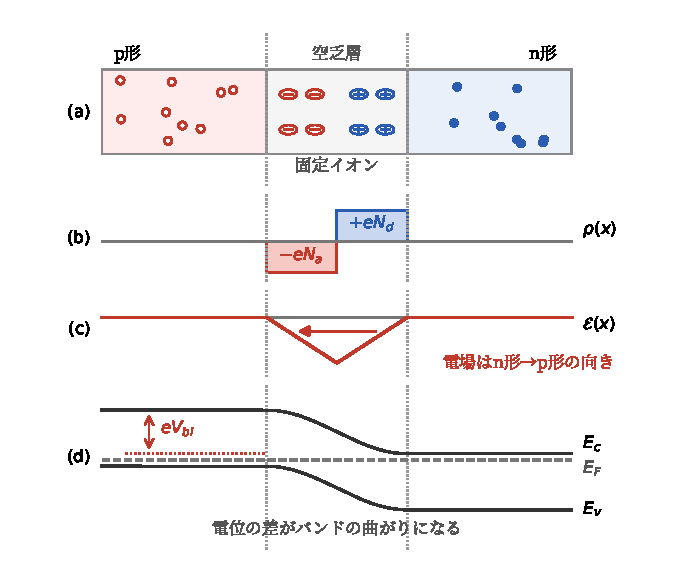
\includegraphics[clip]{figures/fig1.4.eps}
\end{center}
\caption{pn接合と空乏層。(a)拡散と再結合で固定イオンが露出し，(b)電荷密度$\rho(x)$が
(c)電場$\mathcal{E}(x)$を作り，(d)電位の差がバンドの曲がりとして現れる}
\label{fig1.4}
\end{figure}

ここからは電磁気学の出番である。
空乏層には正負の固定電荷が向かい合って分布している（\ref{fig1.4}(b)）。
電荷密度$\rho(x)$があれば，ガウスの法則により電場が生じる。
1次元では
\begin{equation}
\frac{d\mathcal{E}}{dx} = \frac{\rho(x)}{\varepsilon}
\label{eq1.8}
\end{equation}
である（$\varepsilon$は半導体の誘電率）。
電場は正電荷（n形側のドナーイオン）から負電荷（p形側のアクセプタイオン）へ，
つまり\textbf{n形からp形へ向かう}（\ref{fig1.4}(c)）。
この電場を内蔵電場という。
内蔵電場は，電子をn形側へ，正孔をp形側へ押し戻す向きである。
つまり\textbf{拡散をせき止める向き}に働く。
拡散でキャリアが移るほど固定電荷が増えて電場が強まり，
やがて拡散の流れと電場による引き戻し（ドリフト）がちょうど釣り合って，
正味の電流がゼロの平衡状態に落ち着く。

\subsection{バンドの曲がりと拡散電位}

電場があれば電位差がある。電場と電位$\phi$の関係$\mathcal{E} = -d\phi/dx$より，
電位は電場の向きと逆にたどると高くなるから，\textbf{n形側が高くp形側が低い}。
この電位差を\index{かくさんでんい@拡散電位}\textbf{拡散電位}
（内蔵電位）$V_{bi}$という。

電子（電荷$-e$）のポテンシャルエネルギーは$-e\phi$だから，
電位の高いn形側では電子のエネルギーは\textbf{低く}，p形側では\textbf{高い}。
バンド図の縦軸は電子のエネルギーなので，バンドの端は
\begin{equation}
E_c(x) = \text{一定} - e\phi(x)
\label{eq1.9}
\end{equation}
のように電位の分布を上下反転した形になる。
これが\ref{fig1.4}(d)の\textbf{バンドの曲がり}であり，
曲がりの高さは$eV_{bi}$に等しい。
「電荷分布→電場→電位→バンドの曲がり」という一本道で，
バンド図は電磁気学から描けるのである。

\begin{注意}
熱平衡では，バンドは曲がるが\textbf{フェルミ準位は曲がらず水平}である。
もし$E_F$に場所による差があれば，電子は高い方から低い方へ移動し，
電流が流れてしまう。それは平衡ではない。
バンドを容器の底の形，フェルミ準位を水面と思えばよい。
つながった水の水面は，底の形によらず同じ高さになる。
\end{注意}

拡散電位は，接合前のn形とp形のフェルミ準位の差を$e$で割ったものであり，
ドーピング濃度を使うと次のように表せる（導出は2章で行う）。
\begin{equation}
V_{bi} = \frac{kT}{e} \ln\frac{N_a N_d}{n_i^2}
\label{eq1.10}
\end{equation}

\begin{例題}[拡散電位]
\label{rei1.3}
室温のシリコンpn接合で$N_a = N_d = 10^{16}\,\mathrm{cm^{-3}}$のとき，
拡散電位$V_{bi}$を求めよ。
$kT/e = 0.026$\,V，$n_i = 1.5\times10^{10}\,\mathrm{cm^{-3}}$とする。
\begin{解答}
式\ref{eq1.10}より
\begin{eqnarray}
V_{bi} &=& 0.026 \times \ln\frac{10^{16}\times10^{16}}{(1.5\times10^{10})^2}
= 0.026 \times \ln(4.4\times10^{11}) \nonumber\\
&\approx& 0.026 \times 26.8 \approx 0.70\,\mathrm{V} \nonumber
\end{eqnarray}
シリコンのpn接合の拡散電位は，ドーピング濃度によらずおおむね0.6〜0.8\,Vである。
対数はけたが大きく変わっても値があまり変わらないからである。
ダイオードの順方向電圧約0.7\,V（2章）の正体がこの値である。
\end{解答}
\end{例題}

\subsection{空乏層の幅と電場の強さ}

空乏層の幅$d$は，式\ref{eq1.8}を積分すると求められ
（章末問題\ref{ex1.4}で導出する），
\begin{equation}
d = \sqrt{\frac{2\varepsilon V_{bi}}{e}\left(\frac{1}{N_a}+\frac{1}{N_d}\right)}
\label{eq1.11}
\end{equation}
となる。ドーピング濃度が低いほど空乏層は広い。
同じ電荷を集めるのに，キャリアの薄い領域では広い範囲のイオンが必要だからである。
また，濃度に差があるときは\textbf{濃度の低い側に深く広がる}。

空乏層は電圧を受け持つ層である。
空乏層内の電場には上限があり（この上限が
\index{ぜつえんはかいでんかい@絶縁破壊電界}\textbf{絶縁破壊電界}，
シリコンで約$3\times10^7$\,V/m），
これを超えるとなだれのようにキャリアが増えて絶縁が破れる（降伏）。
高い電圧に耐えるには，低濃度で広い空乏層を作って電場を薄く広く分担させるしかない。
ところが低濃度の層は例題\ref{rei1.2}で見たとおり抵抗が大きい。
\textbf{耐圧を取ればオン抵抗が増える} ―
このトレードオフがパワーデバイス設計の中心問題であり，
ワイドギャップ半導体が注目される理由でもある（3章）。

\subsection{バイアスと整流性}

pn接合に外から電圧をかける（バイアスする）と何が起こるか（\FIGref{fig1.5}）。
p形側を正にする電圧（\index{じゅんばいあす@順バイアス}\textbf{順バイアス}）$V$をかけると，
外部電圧は内蔵電場を打ち消す向きに働き，障壁は$e(V_{bi}-V)$に下がる。
障壁を越えられるキャリアが急増し，電流が流れる。
逆にp形側を負にする電圧（\index{ぎゃくばいあす@逆バイアス}\textbf{逆バイアス}）では
障壁が$e(V_{bi}+V)$に上がり，空乏層も広がって，電流はほとんど流れない。

\begin{figure}[ht]
\begin{center}
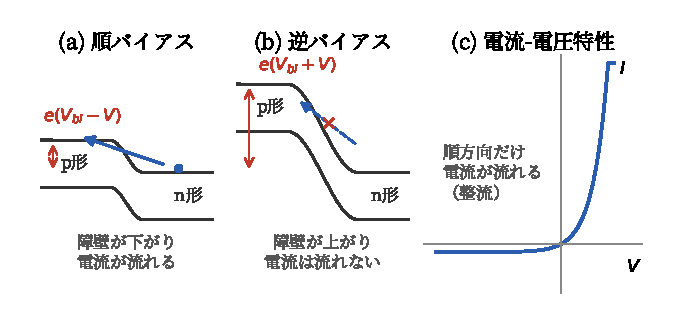
\includegraphics[clip]{figures/fig1.5.eps}
\end{center}
\caption{バイアスとpn接合の整流性。(a)順バイアスでは障壁が下がって電流が流れ，
(b)逆バイアスでは障壁が上がって電流が止まる。(c)一方向にだけ電流を流す}
\label{fig1.5}
\end{figure}

一方向にだけ電流を流すこの性質を
\index{せいりゅうさよう@整流作用}\textbf{整流作用}という。
pn接合は，電圧の向きだけでオンとオフが決まる最も簡単なスイッチ ―
ダイオードそのものである。
電流と電圧の関係式，および逆バイアスへ切り替えた瞬間に流れる逆向きの電流
（逆回復。少数キャリアの引き抜きによる）は2章で扱う。

\begin{問}
\item 式\ref{eq1.11}の右辺の単位がmになることを確かめよ。
誘電率$\varepsilon$の単位はF/m，濃度の単位はm$^{-3}$とし，
$1\,\mathrm{F} = 1$\,C/Vを使ってよい。
\end{問}

%%======================================================================
\section{金属-半導体接合}
\label{sec1.7}

\subsection{素子は必ず金属と接合される}

どんな半導体素子も，最後は金属の電極と配線で外部回路につながる。
つまり素子の中には必ず金属と半導体の接合面がある。
この接合は，作り方しだいで性質がまったく異なる2種類に分かれる。

\begin{箇条書}
\item \textbf{整流性接触}：一方向にしか電流を流さない（ショットキー接合）
\item \textbf{オーミック接触}：どちら向きにも低抵抗で電流を流す（電極に必要）
\end{箇条書}

どちらになるかを決めるのが，次の2つの量である。

\begin{定義}[仕事関数と電子親和力]
\label{def1.4}
物質の外（真空準位）を基準として，
\begin{箇条書}
\item \index{しごとかんすう@仕事関数}\textbf{仕事関数}$\phi_m$，$\phi_s$：
フェルミ準位から電子1個を物質の外へ取り出すのに要するエネルギー
（添字mは金属，sは半導体）
\item \index{でんししんわりょく@電子親和力}\textbf{電子親和力}$\chi_s$：
伝導帯の下端から電子1個を外へ取り出すのに要するエネルギー
\end{箇条書}
$\chi_s$は半導体材料で決まる定数だが（シリコンで$4.05$\,eV），
$\phi_s$はフェルミ準位の位置，つまりドーピングによって変わる。
\end{定義}

\subsection{接合するとバンドが曲がる}

仕事関数の異なる金属と半導体を接合すると，pn接合と同じ筋書きが始まる。
フェルミ準位の高い（仕事関数の小さい）側から低い側へ電子が移り，
界面に電荷がたまり，電場が生じ，半導体側のバンドが曲がる。
曲がりが両者のフェルミ準位の差をちょうど埋めたところで移動が止まり，
フェルミ準位が全体で水平な平衡に達する。

曲がるのはほとんど半導体側だけである。
金属の電子密度（$10^{22}$〜$10^{23}\,\mathrm{cm^{-3}}$）は半導体のキャリア密度より
けた違いに大きく，少々電子が出入りしてもフェルミ準位が動かないからである。
大きな水槽（金属）と小さなコップ（半導体）をつないだとき，
水位がほぼコップ側だけ変わって水槽の水位にそろうのと同じである。

\subsection{ショットキー接合とオーミック接合}

n形半導体との接合を考える。
$\phi_m > \phi_s$なら，電子は半導体から金属へ移る。
半導体の界面付近には電子のいない空乏層（ドナーイオンの正の固定電荷）ができ，
バンドが上に曲がって，電子の行く手をはばむエネルギー障壁ができる。
この障壁を\index{しょっときーしょうへき@ショットキー障壁}\textbf{ショットキー障壁}といい，
金属側から見た高さは
\begin{equation}
\phi_B = \phi_m - \chi_s
\label{eq1.12}
\end{equation}
である。
障壁のあるこの接合は
\index{しょっときーせつごう@ショットキー接合}\textbf{ショットキー接合}と呼ばれ，
pn接合と同様の整流性を示す。
順方向電圧がpn接合より小さく（0.3〜0.4\,V），
少数キャリアを使わないため逆回復が速い ―
ショットキーバリアダイオードとしての使いどころは3章で述べる。

$\phi_m < \phi_s$なら電子は金属から半導体へ移り，
界面の電子はかえって増えるから障壁はできず，
どちら向きにも低抵抗で電流が流れる
\index{おーみっくせつごう@オーミック接合}\textbf{オーミック接合}になる。

p形半導体では多数キャリアが正孔なので，同じ大小関係で結果が逆になる
（\TABref{tab1.1}）。

\begin{table}[ht]
\begin{center}
\caption{金属-半導体接合の型。仕事関数の大小と半導体の形で決まる}
\label{tab1.1}
\begin{tabular}{c|c|c}
\hline
仕事関数の関係 & n形半導体 & p形半導体 \\
\hline
$\phi_m > \phi_s$ & 整流性（ショットキー） & オーミック \\
$\phi_m < \phi_s$ & オーミック & 整流性（ショットキー） \\
\hline
\end{tabular}
\end{center}
\end{table}

実際の素子の電極では，仕事関数の合う金属を選ぶだけでなく，
半導体の表面を高濃度（$10^{19}\,\mathrm{cm^{-3}}$以上）にドーピングする方法が広く使われる。
濃度が高いと空乏層が式\ref{eq1.11}のとおり数nmまで薄くなり，
電子が障壁をすり抜けて（トンネル効果），
仕事関数の関係によらずオーミック接合が得られるからである。

これで役者がそろった。
pn接合と金属-半導体接合を組み合わせれば，
ダイオード・MOSFET・IGBTといったパワー半導体デバイスが組み上がる。
2章では，これらの素子が「なぜスイッチとして動くのか」を本章の物理から導く。

\begin{問}
\item 金（仕事関数$\phi_m = 5.1$\,eV）とn形シリコン（仕事関数$\phi_s = 4.3$\,eV，
電子親和力$\chi_s = 4.05$\,eV）の接合は，ショットキー接合とオーミック接合の
どちらになるか。整流性をもつ場合はショットキー障壁の高さも求めよ。
\end{問}

%%======================================================================
\begin{章末問題}
\item \label{ex1.1}
式\ref{eq1.2}で$E - E_F \gg kT$のとき$f(E) \approx \exp\left(-\frac{E-E_F}{kT}\right)$と
近似できることを示せ。
さらに室温（$kT = 0.026$\,eV）において，
フェルミ準位がバンドギャップ中央にあるとして，
伝導帯下端（$E - E_F = E_g/2$）の占有確率をシリコン（$E_g = 1.1$\,eV）と
SiC（$E_g = 3.3$\,eV）について概算し，比を比較せよ。
この結果から，SiCデバイスの漏れ電流と高温動作について何がいえるか。

\item \label{ex1.2}
n形シリコンにドナーを$N_d = 10^{17}\,\mathrm{cm^{-3}}$だけドーピングした。
$n_i = 1.5\times10^{10}\,\mathrm{cm^{-3}}$，
$\mu_n = 1350\,\mathrm{cm^2/(V\cdot s)}$とする。
\begin{enumerate}
\item[(a)] 電子濃度$n$と正孔濃度$p$を求めよ。
\item[(b)] 導電率$\sigma$を求めよ。正孔の寄与は無視してよい。
\end{enumerate}

\item \label{ex1.3}
室温のシリコンpn接合で$N_a = N_d = 10^{16}\,\mathrm{cm^{-3}}$とする。
シリコンの誘電率は$\varepsilon = 11.7\varepsilon_0$
（$\varepsilon_0 = 8.854\times10^{-12}$\,F/m），
拡散電位は例題\ref{rei1.3}の$V_{bi} = 0.70$\,Vとする。
\begin{enumerate}
\item[(a)] 空乏層幅$d$を式\ref{eq1.11}から求めよ。
\item[(b)] 空乏層内の電場は接合面で最大になる。
対称接合では最大電場が$\mathcal{E}_{\max} = 2V_{bi}/d$と書けることを使って
$\mathcal{E}_{\max}$を求め，シリコンの絶縁破壊電界$3\times10^7$\,V/mと比較せよ。
\end{enumerate}

\item \label{ex1.4}
式\ref{eq1.11}を導出しよう。
p形側$-x_p < x < 0$に$\rho = -eN_a$，n形側$0 < x < x_n$に$\rho = +eN_d$の
固定電荷が一様に分布し，空乏層の外に電場はないとする。
\begin{enumerate}
\item[(a)] 空乏層の外の電場がゼロであることから，
$N_a x_p = N_d x_n$（電荷のつり合い）を示せ。
\item[(b)] 式\ref{eq1.8}を積分し，電場の大きさが接合面$x=0$で
最大となる三角形の分布になることを示せ。
また最大値が$\mathcal{E}_{\max} = eN_a x_p/\varepsilon$
（$= eN_d x_n/\varepsilon$）と書けることを確かめよ。
\item[(c)] 電位差は電場の分布の面積に等しい
（$V_{bi} = \frac{1}{2}\mathcal{E}_{\max}d$，$d = x_p + x_n$）。
これらから式\ref{eq1.11}を導け。
\end{enumerate}

\item \label{ex1.5}
SiCやGaNなどのワイドギャップ半導体がパワーエレクトロニクスで注目される理由を，
(a)真性キャリア濃度，(b)絶縁破壊電界の2つの観点から，
本章で学んだ物理に基づいて説明せよ。
\end{章末問題}
